\section{Implementation of the test suite}
\label{section:test_suite}

\subsection{Core architecture}

\paragraph{}
The architecture of the benchmarking test suit is designed in a rather simple manner such that it permits easy addition of more test cases or graph sketches. It is shown in \autoref{fig:test_suite}.

\begin{figure}[H]
    \centering 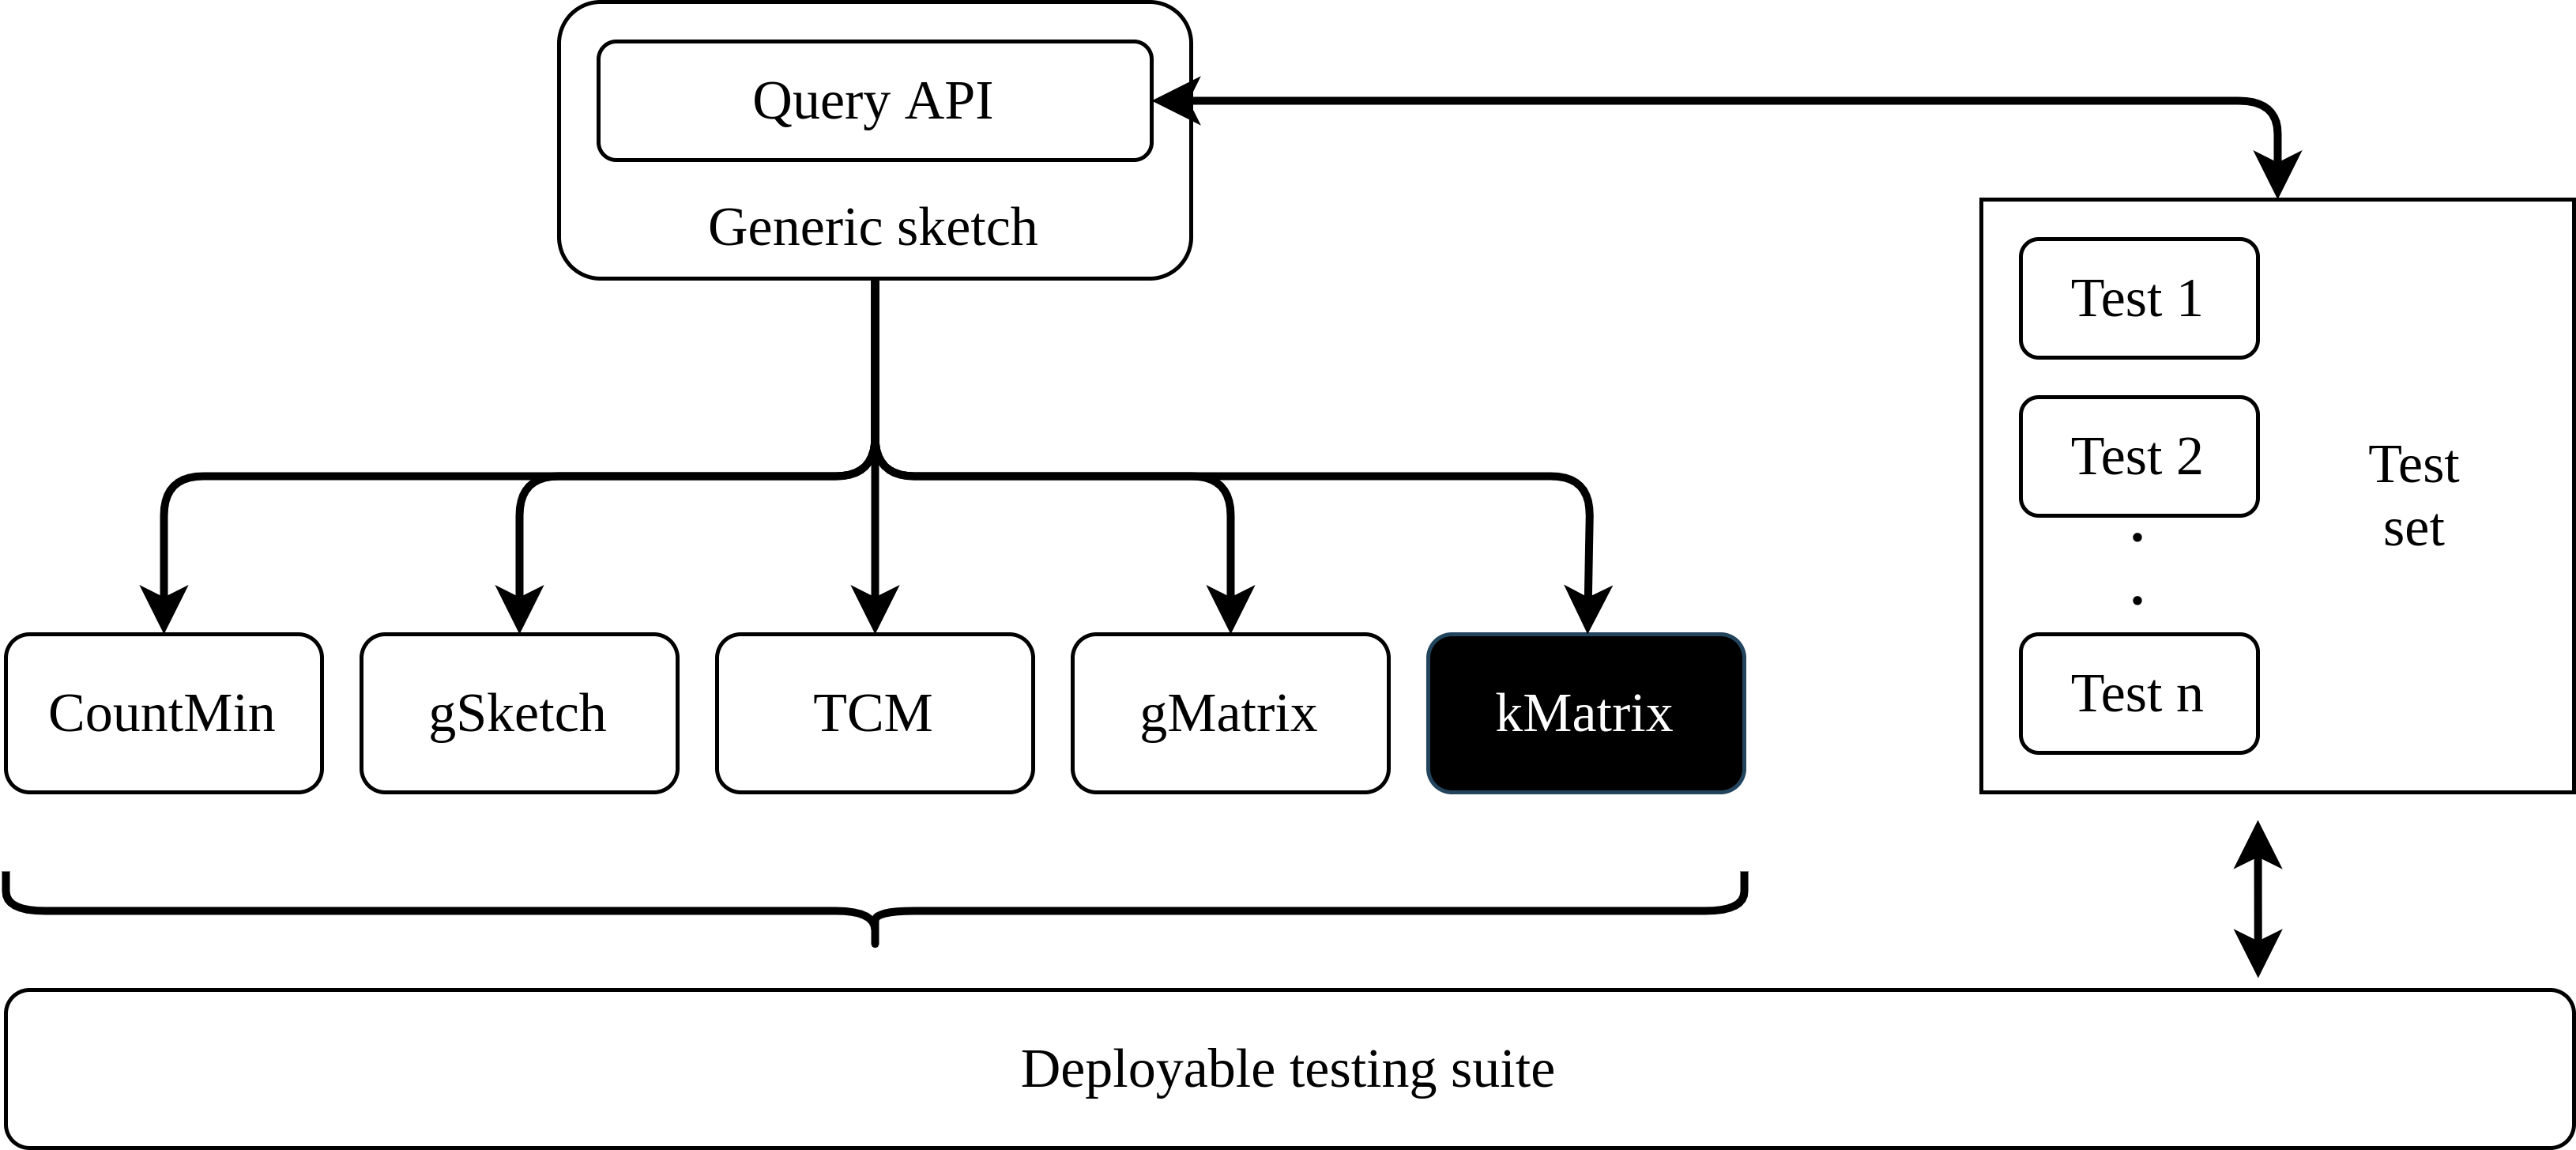
\includegraphics[width=\textwidth]{test_suite}
    \caption{High level architecture of the test suite}
    \label{fig:test_suite}
\end{figure}

\paragraph{}
All the sketches are extended from a generic ‘Sketch’ class which allows the tests to retrieve information through a same interface. This class contains the abstract methods \textbf{add\_edge{()}}, \textbf{get\_edge\_frequency{()}} and \textbf{print\_analytics{()}}. They were to be implemented by any of the sketches that inherit from the base Sketch class. The code for the base Sketch class is depicted in \autoref{lst:sketch}.\\

\pythonexternal[caption={Sketch class}, label={lst:sketch}]{code_listings/sketch.py}

\subsection{Utility functions}

\paragraph{}
All the utility functions were implemented in a separate Python module. The reservoir sampling of data streams was done using the sampling function depicted in \autoref{lst:sampling}.

\pythonexternal[caption={Reservoir sampling function}, label={lst:sampling}]{code_listings/sampling.py}

\paragraph{}
The \textbf{timeit} function used for the timing of code sections can be found in the appendix \ref{appendix:timeit}.

\subsection{Summarization sketches}

\paragraph{}
Restating the aforementioned, all the summarization sketches have been extended from the base Sketch class. The implementation code for the sketches, CountMin, gSketch, TCM and GMatrix can be found respectively in \ref{appendix:countmin}, \ref{appendix:gsketch}, \ref{appendix:tcm} and \ref{appendix:gmatrix} appendix sections.